\section{Durchführung}
Der Versuchsaufbau besteht aus einer Steckplatine, an die ein Oszilloskop und ein Funktionsgenerator angeschlossen werden können, sowie verschiedenen Elektronikbauteilen. Der exakte Aufbau der einzelnen Versuchsteile wird in den folgenden Abschnitten beschrieben.


\subsection{Invertierender Linearverstärker}
Es wird ein wie in \autoref{fig:Umkehr} abgebildeter invertierender gegengekoppelter Linearverstärker aufgebaut. Der Frequenzgang des Verstärkers wird für mindestens vier Verstärkungsgrade gemessen. (Die Verstärkung fällt mit steigender Frequenz bei sinusförmigen Eingangssignalen ab.) 
Die Phase zwischen Ein- und Ausgangssignal wird in Abhängigkeit des Widerstandsverhältnisses und der Frequenz gemessen.

\begin{figure}
    \centering
    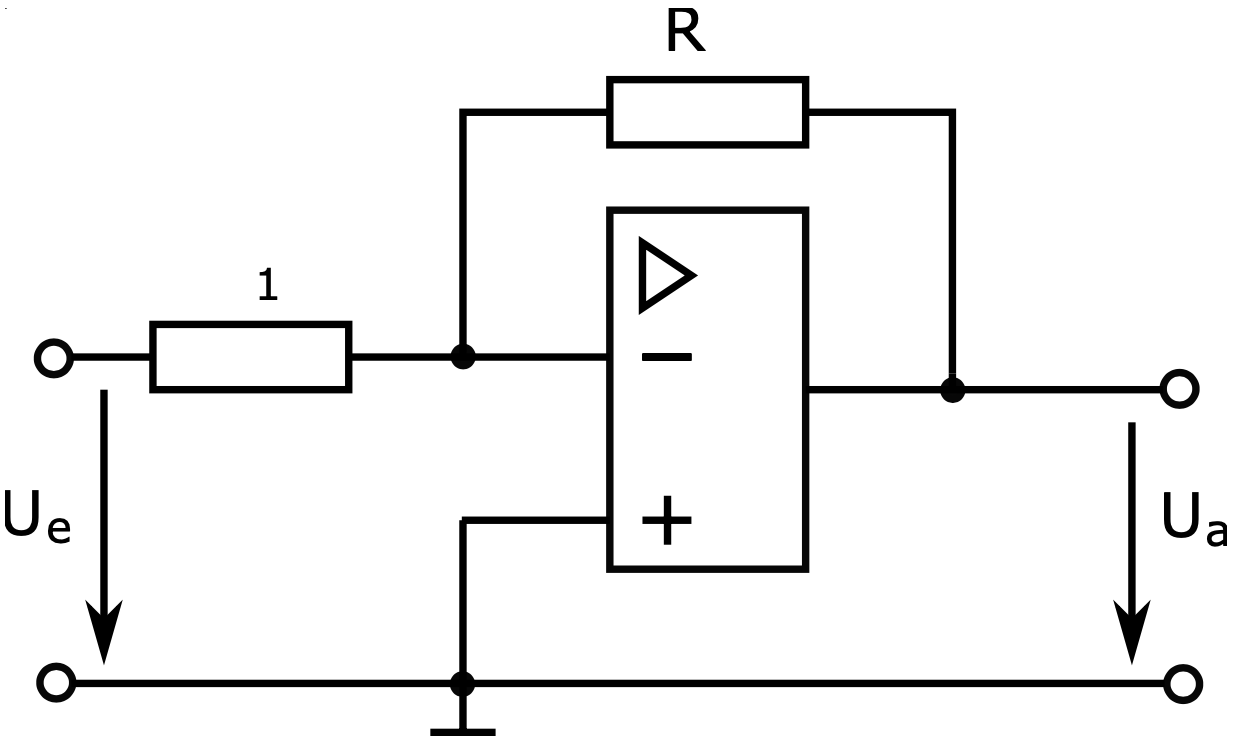
\includegraphics[width=0.7\linewidth]{./figures/1_InvLinear.png}
    \caption{Aufbau. \cite{Anleitung}}
    \label{fig:InvLinear}
\end{figure}


\subsection{Umkehr-Integrator}
\label{sec:Umkehr}
Der in \autoref{fig:Umkehr} gezeigte Umkehr-Integrator wird aufgebaut.
Es wird die Ein- und Ausgangsspannung in Abhängigkeit der Frequenz gemessen. Das Eingangssignal ist dabei sinusförmig.
%Es wird die Proportionalität zwischen der Ausgangsspannung und dem Kehrwert der Frequenz für ein sinusförmiges Eingangssignal gemessen und so überprüft, dass die gewählte Zeitkonstante sinnvoll ist.

Es werden ein Bildschirmfoto sowie die Daten der Ausgangssignale am Oszilloskop für sinusförmige, dreieckförmige und rechteckförmige Eingangssignale gespeichert.

\begin{figure}
    \centering
    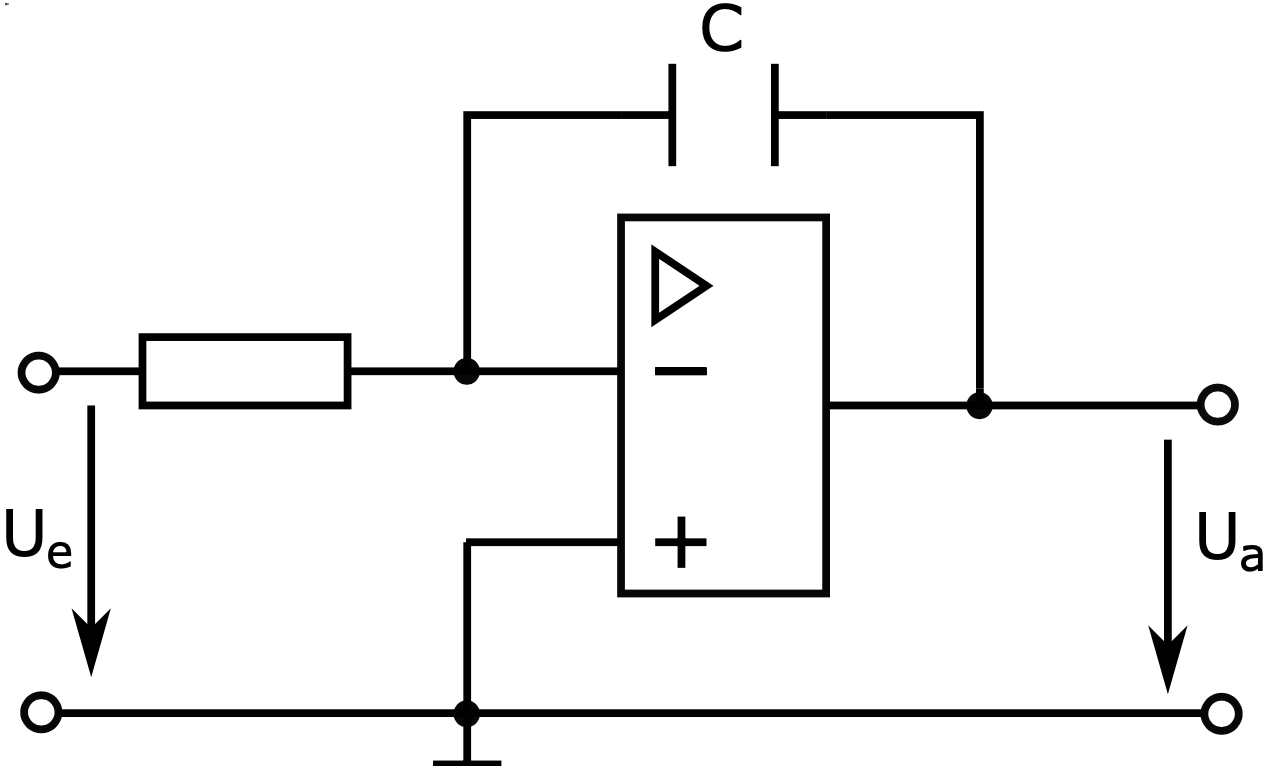
\includegraphics[width=0.7\linewidth]{./figures/2_Umkehr.png}
    \caption{Aufbau. \cite{Anleitung}}
    \label{fig:Umkehr}
\end{figure}


\subsection{Invertierender Differenzierer}
In diesem Versuchsteil wird die Schaltung aus \autoref{fig:InvDiff} aufgebaut und die Schritte aus \autoref{sec:Umkehr} wiederholt.

\begin{figure}
    \centering
    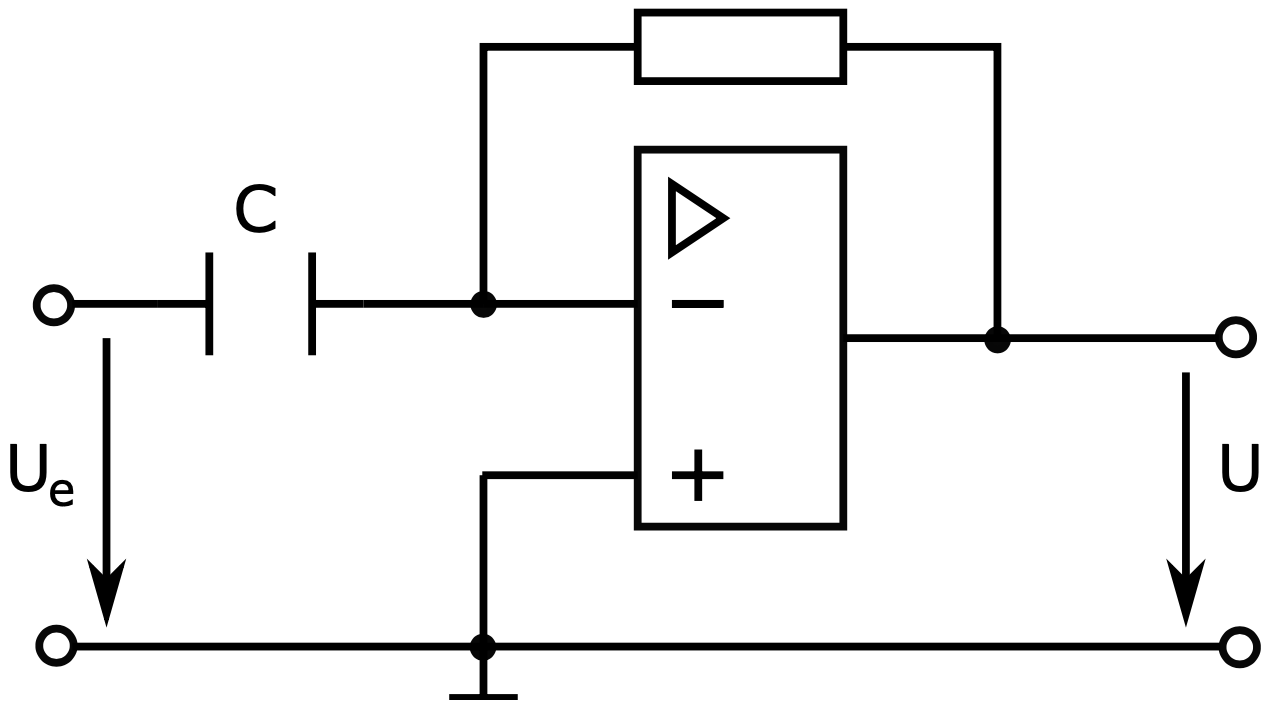
\includegraphics[width=0.7\linewidth]{./figures/3_InvDiff.png}
    \caption{Aufbau. \cite{Anleitung}}
    \label{fig:InvDiff}
\end{figure}


\subsection{Nicht-invertierende Schmitt-Trigger}
\label{sec:Schmitt}
Die in \autoref{fig:Schmitt} abgebildete Schmitt-Trigger-Schaltung wird aufgebaut und es wird ein sinusförmiges Eingangssignal angelegt. Die Amplitude wird von $\SI{0}{\volt}$ bis \dots in $\SI{1}{\milli\volt}$-Schritten erhöht. %Schrittweite Wert ändern
Die Amplitude, bei der die Schaltung beginnt zu kippen, wird bestimmt.
%Alternativ: Dreieckssignal

Am Oszilloskop werden synchrone Daten von Ein- und Ausgangsspannung gespeichert.
 %Hysterese-Verlaufskurve

\begin{figure}
    \centering
    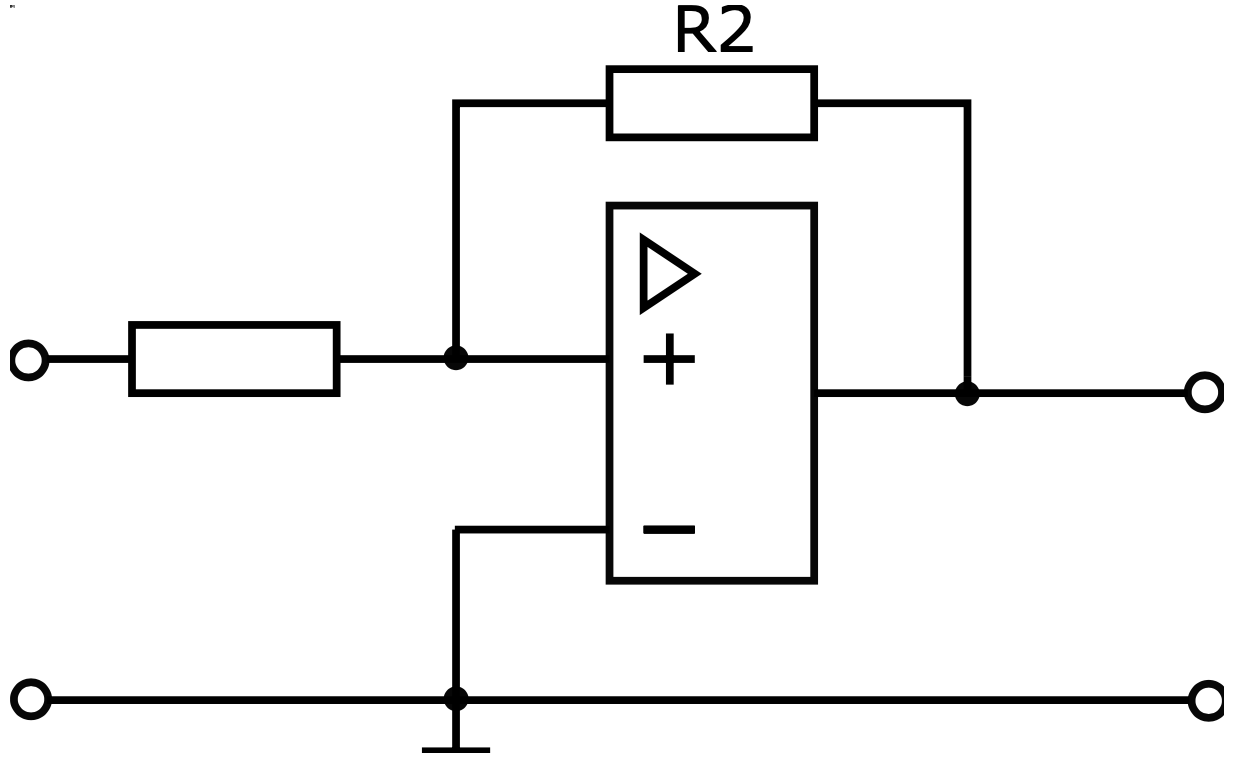
\includegraphics[width=0.7\linewidth]{./figures/4_Schmitt.png}
    \caption{Aufbau. \cite{Anleitung}}
    \label{fig:Schmitt}
\end{figure}


\subsection{Signalgenerator}
Hinter die in \autoref{sec:Schmitt} gezeigte Schmitt-Trigger-Schaltung wird ein Integrator gebaut (siehe \autoref{fig:Signal}). Das Eingangssignal ist sinusförmig und das Ausgangssignal dreiecksförmig. Die Frequenz und deren Amplitude der erzeugten Schwingung wird bestimmt. 

\begin{figure}
    \centering
    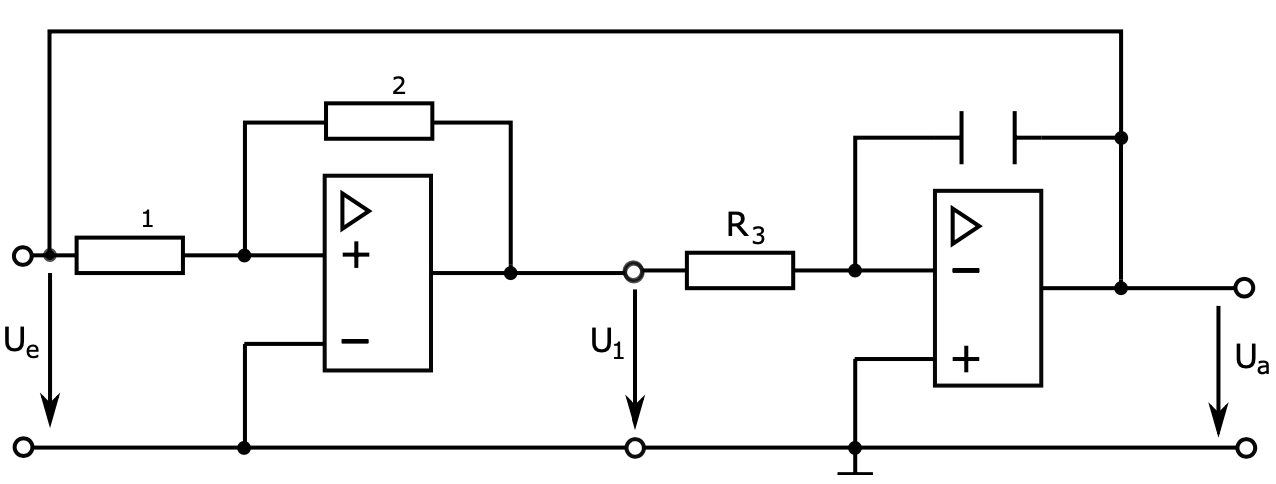
\includegraphics[width=0.7\linewidth]{./figures/5_Signal.png}
    \caption{Aufbau. \cite{Anleitung}}
    \label{fig:Signal}
\end{figure}


\subsection{Variierende Amplituden}
Die Schaltung für variierende Amplituden wird wie in \autoref{fig:VarAmp} aufgebaut. Der Wert für die Kapazität ist $C = \SI{20}{\nano\farad}$. %oder 100
Die Dämpfung/ Enddämpfung kann am Potentiometer P zwischen -1 und 1 variiert werden.
Die \autoref{eq:SchwingAbkling} soll nachgewiesen werden.

Für den Fall, dass $\eta < 0$ ist, wird eine gedämpfte Schwingung mit dem Oszilloskop aufgenommen. Hier muss zusätzlich eine Rechteckspannung eingespeist werden, da das System nicht von selbst schwingt.

Für den Fall, dass $\eta > 0$ ist, wird eine charakteristische Frequenz/ Schwingungsdauer ausgemessen.

\begin{figure}
    \centering
    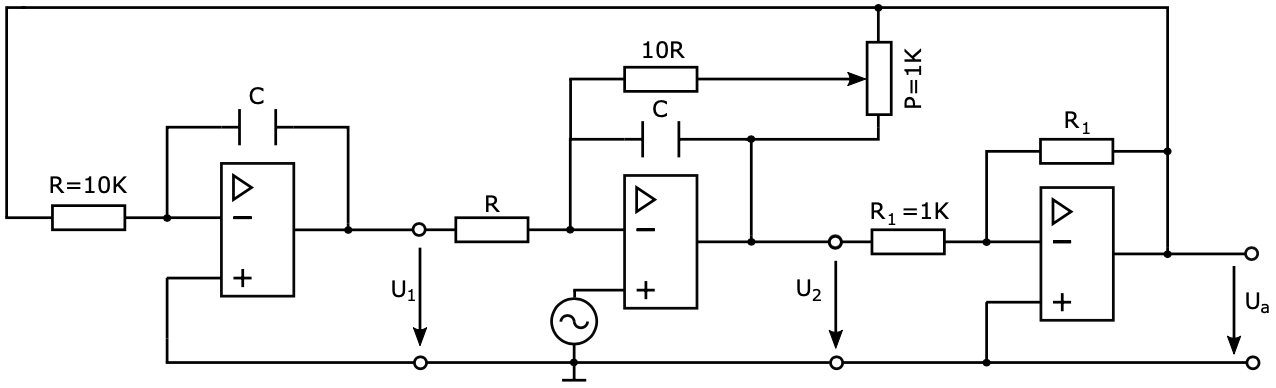
\includegraphics[width=0.7\linewidth]{./figures/6_VarAmp.png}
    \caption{Aufbau. \cite{Anleitung}}
    \label{fig:VarAmp}
\end{figure}